\chapter{Phân tích và thiết kế hệ
thống}\label{phuxe2n-tuxedch-vuxe0-thiux1ebft-kux1ebf-hux1ec7-thux1ed1ng}

\section{Phân tích yêu cầu}\label{phuxe2n-tuxedch-yuxeau-cux1ea7u}

\subsection{Yêu cầu chức
năng}\label{yuxeau-cux1ea7u-chux1ee9c-nux103ng}

\subsubsection{Quản lý dữ liệu đầu
vào}\label{quux1ea3n-luxfd-dux1eef-liux1ec7u-ux111ux1ea7u-vuxe0o}

Hệ thống cần cung cấp khả năng nhập liệu đa dạng để tập trung tri thức
từ các nguồn phân tán và biến hệ thống thành "second brain" cho doanh
nghiệp F\&B.

\begin{itemize}
\item
  Mô tả:

  \begin{itemize}
  \item
    Tải lên Tài liệu phi cấu trúc: Cho phép người dùng tải lên (upload)
    các tài liệu như:

    \begin{itemize}
    \item
      File PDF (hợp đồng, báo cáo doanh số, menu, tài liệu đối tác).
    \item
      File Word/Docx (quy trình vận hành, chính sách nhân sự).
    \item
      File Text/Markdown (ghi chú nhanh, ý tưởng công thức mới).
    \end{itemize}
  \item
    Nhập liệu từ Đường dẫn (URL): Hỗ trợ nhập URL để thu thập nội dung
    từ các bài blog chuyên ngành F\&B, bài viết về xu hướng ẩm thực,
    hoặc trang web đối thủ cạnh tranh.
  \item
    Hỗ trợ Transcript: Cho phép nhập văn bản thô từ transcript của các
    cuộc họp nội bộ hoặc các video hướng dẫn làm món ăn.
  \end{itemize}
\item
  Yêu cầu kỹ thuật:

  \begin{itemize}
  \item
    Hệ thống phải kiểm tra định dạng và kích thước file hợp lệ (ví dụ:
    tối đa 50MB) trước khi cho phép xử lý.
  \item
    Cần có khả năng xử lý và mã hóa văn bản chính xác cho cả tiếng Việt
    và tiếng Anh.
  \item
    Ưu tiên phát triển tiện ích trình duyệt (browser extension) để lưu
    trữ nhanh chóng các nội dung từ Internet.
  \end{itemize}
\end{itemize}

\subsubsection{Trích xuất và xử lý tri
thức}\label{truxedch-xuux1ea5t-vuxe0-xux1eed-luxfd-tri-thux1ee9c}

Chức năng này đảm bảo dữ liệu phi cấu trúc được chuyển hóa thành định
dạng có thể truy vấn và sử dụng hiệu quả bởi mô hình AI (phục vụ cho
RAG).

\begin{itemize}
\item
  Mô tả:

  \begin{itemize}
  \item
    Phân tích và Trích xuất: Tự động phân tích và trích xuất các thành
    phần quan trọng (ví dụ: ngày tháng, từ khóa, tên món, giá cả, chủ đề
    chính) từ nội dung đã tải lên.
  \item
    Phân đoạn (Chunking): Chia nhỏ các tài liệu lớn thành các đoạn văn
    bản (chunks) có kích thước tối ưu (ví dụ: 256--512 token) để đảm bảo
    độ chính xác khi tìm kiếm.
  \item
    Mã hóa (Embedding): Sử dụng các mô hình embedding (ví dụ: BGE, E5)
    để chuyển đổi các đoạn văn bản thành vector số học và lưu trữ chúng
    vào Vector Database.
  \item
    Xử lý hình ảnh/phi văn bản: Tích hợp OCR (Optical Character
    Recognition) để xử lý các file PDF dạng scan hoặc hình ảnh chứa văn
    bản (ví dụ: chụp lại menu viết tay).
  \end{itemize}
\item
  Yêu cầu kỹ thuật:

  \begin{itemize}
  \item
    Đảm bảo tốc độ xử lý nhanh và tính năng xử lý diễn ra ngầm
    (background service) để không ảnh hưởng đến trải nghiệm người dùng.
  \item
    Phải có cơ chế kiểm tra trùng lặp (duplication check) vector để
    tránh lãng phí tài nguyên và làm giảm chất lượng truy vấn.
  \end{itemize}
\end{itemize}

\subsubsection{Xây dựng và quản lý Cơ sở Tri thức (Knowledge
Base)}\label{xuxe2y-dux1ef1ng-vuxe0-quux1ea3n-luxfd-cux1a1-sux1edf-tri-thux1ee9c-knowledge-base}

Quản lý tập trung và hiệu quả kho tri thức của doanh nghiệp (Internal
Knowledge) và dữ liệu xu hướng công khai.

\begin{itemize}
\item
  Mô tả:

  \begin{itemize}
  \item
    Tổ chức dữ liệu: Cho phép người dùng quản lý tài liệu theo không
    gian làm việc (Workspace) hoặc theo dự án/chi nhánh (Project) để
    phân loại tri thức.
  \item
    Cập nhật Tri thức: Cung cấp cơ chế để người dùng cập nhật lại vector
    hoặc đánh dấu phiên bản cũ khi có phiên bản mới của tài liệu được
    tải lên.
  \item
    Quản lý Trạng thái: Hiển thị trạng thái xử lý của từng tài liệu
    (Đang xử lý, Đã Index xong, Xảy ra lỗi).
  \item
    Làm giàu dữ liệu: Có module thu thập dữ liệu xu hướng công khai
    (trending hashtags, popular sounds/music trên TikTok/Reels, sự kiện
    lớn của ngành F\&B) để làm giàu nguồn dữ liệu đầu vào cho AI Agent.
  \end{itemize}
\item
  Yêu cầu kỹ thuật:

  \begin{itemize}
  \item
    Hỗ trợ đầy đủ các thao tác CRUD (Create, Read, Update, Delete) đối
    với các tài liệu và cấu trúc tổ chức (Workspace, Project).
  \item
    Sử dụng Vector Database chuyên dụng (ví dụ: ChromaDB, Pinecone) để
    lưu trữ các embedding một cách hiệu quả.
  \end{itemize}
\end{itemize}

\subsubsection{Truy xuất thông tin bằng ngôn ngữ tự nhiên
(RAG)}\label{truy-xuux1ea5t-thuxf4ng-tin-bux1eb1ng-nguxf4n-ngux1eef-tux1ef1-nhiuxean-rag}

Đây là chức năng giao tiếp cốt lõi, cho phép người dùng không chuyên kỹ
thuật có thể tương tác với kho tri thức của mình một cách dễ dàng và
chính xác.

\begin{itemize}
\item
  Mô tả:

  \begin{itemize}
  \item
    Truy vấn Ngôn ngữ tự nhiên: Người dùng đặt câu hỏi bằng ngôn ngữ tự
    nhiên (ví dụ: "Chiến lược giá của combo A là gì?" hoặc "Thông tin về
    sản phẩm cà phê mới nằm ở đâu?").
  \item
    Thực thi RAG: Hệ thống tự động chuyển câu hỏi thành truy vấn vector,
    tìm kiếm các đoạn văn bản liên quan nhất từ Cơ sở Tri thức, và đưa
    chúng vào LLM để tạo ra câu trả lời tổng hợp.
  \end{itemize}
\end{itemize}

\begin{itemize}
\item
  Yêu cầu kỹ thuật:

  \begin{itemize}
  \item
    Đảm bảo độ trễ truy vấn thấp (latency).
  \item
    Triển khai kỹ thuật Post-processing và Re-ranking (sắp xếp lại thứ
    tự kết quả) để cải thiện chất lượng của các đoạn văn bản được truy
    xuất.
  \end{itemize}
\end{itemize}

\subsubsection{Chức năng AI Agent hỗ trợ người dùng (Marketing Automation
Core)}\label{chux1ee9c-nux103ng-ai-agent-hux1ed7-trux1ee3-ngux1b0ux1eddi-duxf9ng-marketing-automation-core}

Đây là chức năng giao tiếp cốt lõi, cho phép người dùng tương tác với cơ
sở tri thức bằng ngôn ngữ tự nhiên và sử dụng hệ thống để tạo ra các nội
dung marketing.

\begin{itemize}
\item
  Mô tả:

  \begin{itemize}
  \item
    Truy vấn ngôn ngữ tự nhiên: Người dùng đặt câu hỏi bằng ngôn ngữ tự
    nhiên để truy xuất thông tin từ các tài liệu đã lưu trữ hoặc yêu cầu
    hệ thống tạo ra nội dung marketing.
  \item
    Thực thi RAG: Hệ thống tự động chuyển đổi câu hỏi hoặc yêu cầu thành
    truy vấn vector, tìm kiếm các đoạn văn bản liên quan nhất từ cơ sở
    tri thức, sau đó sử dụng các đoạn văn bản này để tạo ra câu trả lời
    chính xác hoặc nội dung marketing phù hợp.
  \item
    Tạo nội dung marketing: Hệ thống có khả năng tạo ra các nội dung
    marketing dựa trên các tài liệu và nguồn cảm hứng đã lưu trữ, bao
    gồm:
  \item
    Tạo chiến lược nội dung: Đề xuất các chủ đề, ý tưởng và hướng tiếp
    cận cho các chiến dịch marketing
  \item
    Tạo bài nội dung: Tạo các caption, bài viết ngắn và nội dung văn bản
    cho các bài đăng trên mạng xã hội
  \item
    Tạo kịch bản video: Tạo kịch bản chi tiết cho các video ngắn, bao
    gồm cấu trúc nội dung, thông điệp chính và các yếu tố cần thiết
  \end{itemize}
\item
  Yêu cầu kỹ thuật:

  \begin{itemize}
  \item
    Đảm bảo thời gian phản hồi truy vấn thấp
  \item
    Triển khai các kỹ thuật hậu xử lý và sắp xếp lại kết quả để nâng cao
    chất lượng các đoạn văn bản được truy xuất
  \item
    Đảm bảo các nội dung được tạo ra có tính mạch lạc, phù hợp với ngữ
    cảnh và nhất quán về giọng văn
  \end{itemize}
\end{itemize}

\subsubsection{Cảnh báo và nhắc nhở thông tin quan
trọng}\label{cux1ea3nh-buxe1o-vuxe0-nhux1eafc-nhux1edf-thuxf4ng-tin-quan-trux1ecdng}

Đảm bảo người dùng bận rộn trong SME không bỏ lỡ các thông tin hoặc công
việc quan trọng.

\begin{itemize}
\item
  Mô tả:

  \begin{itemize}
  \item
    Thông báo thời gian thực: Gửi thông báo (qua WebSocket) khi một tài
    liệu lớn đã xử lý xong và sẵn sàng để tra cứu, hoặc khi nội dung
    được AI tạo đã sẵn sàng để duyệt.
  \item
    Cảnh báo nghiệp vụ: Dựa trên các mốc thời gian trích xuất được từ
    tài liệu (ví dụ: ngày hết hạn hợp đồng, thời điểm bắt đầu khuyến
    mãi), Agent sẽ tự động gửi email hoặc thông báo nhắc nhở tới nhân
    viên/quản lý.
  \end{itemize}
\item
  Yêu cầu kỹ thuật:

  \begin{itemize}
  \item
    Triển khai dịch vụ lập lịch (Scheduler Service) để kiểm tra và gửi
    thông báo đúng thời điểm.
  \end{itemize}
\end{itemize}

\subsubsection{Quản lý người dùng và phân
quyền}\label{quux1ea3n-luxfd-ngux1b0ux1eddi-duxf9ng-vuxe0-phuxe2n-quyux1ec1n}

Đảm bảo tính bảo mật và quản trị dữ liệu cho các doanh nghiệp có nhiều
nhân viên.

\begin{itemize}
\item
  Mô tả:

  \begin{itemize}
  \item
    Xác thực: Hỗ trợ đăng ký/Đăng nhập qua Email/Mật khẩu và Single
    Sign-On (Google).
  \item
    Phân quyền (RBAC - Role-Based Access Control): Phân chia vai trò rõ
    ràng (ví dụ: Admin có quyền quản lý tài liệu gốc; Manager có quyền
    duyệt bài; Staff chỉ có quyền đọc tri thức).
  \end{itemize}
\item
  Yêu cầu kỹ thuật:

  \begin{itemize}
  \item
    Sử dụng cơ chế bảo mật tiêu chuẩn (ví dụ: JWT, OAuth 2.0).
  \end{itemize}
\end{itemize}

\subsubsection{Ghi nhận và lưu trữ lịch sử sử
dụng}\label{ghi-nhux1eadn-vuxe0-lux1b0u-trux1eef-lux1ecbch-sux1eed-sux1eed-dux1ee5ng}

Lưu trữ và thu thập phản hồi để tối ưu hóa hệ thống và mang lại trải
nghiệm tốt hơn.

\begin{itemize}
\item
  Mô tả:

  \begin{itemize}
  \item
    Lịch sử Tương tác: Lưu trữ lịch sử các đoạn hội thoại
    (Threads/Sessions) giữa người dùng và AI Agent, cho phép người dùng
    đặt tên và xem lại sau này.
  \item
    Thu thập Phản hồi: Cho phép người dùng đánh giá (Like/Dislike hoặc
    đánh giá sao) đối với các câu trả lời của RAG và nội dung do Agent
    tạo ra.
  \end{itemize}
\item
  Yêu cầu kỹ thuật:

  \begin{itemize}
  \item
    Lưu trữ dữ liệu phản hồi có cấu trúc để phục vụ cho việc tinh chỉnh
    mô hình (fine-tuning) trong các giai đoạn phát triển tiếp theo.
  \end{itemize}
\end{itemize}

\subsection{Yêu cầu phi chức
năng}\label{yuxeau-cux1ea7u-phi-chux1ee9c-nux103ng}

\subsubsection{Hiệu năng hệ
thống}\label{hiux1ec7u-nux103ng-hux1ec7-thux1ed1ng}

\begin{itemize}
\item
  Thời gian phản hồi (Latency):

  \begin{itemize}
  \item
    Đối với các truy vấn tìm kiếm thông tin đơn giản: Hệ thống cần trả
    về kết quả trong vòng dưới 3 giây.
  \item
    Đối với các tác vụ phức tạp yêu cầu tổng hợp thông tin (RAG) và sinh
    câu trả lời từ LLM: Thời gian phản hồi không được vượt quá 10 - 15
    giây để tránh làm gián đoạn trải nghiệm người dùng.
  \end{itemize}
\item
  Tốc độ xử lý dữ liệu (Ingestion Speed):

  \begin{itemize}
  \item
    Quá trình upload, trích xuất văn bản (OCR/Parsing) và vector hóa
    (Embedding) tài liệu mới cần được thực hiện ngầm (background task).
    Với tài liệu văn bản dưới 10MB, thời gian khả dụng để tìm kiếm sau
    khi upload nên dưới 1 phút.
  \end{itemize}
\end{itemize}

\subsubsection{Độ chính xác và độ tin
cậy}\label{ux111ux1ed9-chuxednh-xuxe1c-vuxe0-ux111ux1ed9-tin-cux1eady}

\begin{itemize}
\item
  Giảm thiểu ảo giác (Hallucination): Đây là yêu cầu quan trọng nhất đối
  với AI Agent trong doanh nghiệp. Hệ thống chỉ được trả lời dựa trên
  các dữ liệu có trong Knowledge Base (Context). Nếu không tìm thấy
  thông tin, AI phải phản hồi "Không tìm thấy thông tin trong tài liệu"
  thay vì tự bịa đặt.
\item
  Tính nhất quán: Với cùng một câu hỏi và cùng một bộ dữ liệu, hệ thống
  phải đưa ra các câu trả lời có nội dung tương đương nhau, không mâu
  thuẫn.
\item
  Trích dẫn nguồn: Mọi câu trả lời được sinh ra từ quy trình RAG bắt
  buộc phải đi kèm trích dẫn (reference) đến tài liệu gốc (tên file, số
  trang) để người dùng có thể kiểm chứng.
\end{itemize}

\subsubsection{Tính mở rộng}\label{tuxednh-mux1edf-rux1ed9ng}

\begin{itemize}
\item
  Dữ liệu: Cơ sở dữ liệu Vector (Vector Database) cần có khả năng lưu
  trữ và truy xuất hiệu quả khi số lượng tài liệu tăng lên (từ vài trăm
  đến hàng chục nghìn vector) mà không làm giảm đáng kể tốc độ tìm kiếm.
\item
  Người dùng: Kiến trúc hệ thống (Backend) cần được thiết kế để hỗ trợ
  đồng thời nhiều người dùng truy cập (concurrent users) mà không bị tắc
  nghẽn, phù hợp với quy mô SME (từ 10-50 nhân sự).
\item
  Mô hình: Hệ thống cần được thiết kế dạng mô-đun để dễ dàng thay thế
  hoặc nâng cấp mô hình LLM (ví dụ: chuyển từ GPT-3.5 sang GPT-4o hoặc
  Llama 3) khi có nhu cầu về chất lượng cao hơn.
\end{itemize}

\subsubsection{Tính thân thiện với người
dùng}\label{tuxednh-thuxe2n-thiux1ec7n-vux1edbi-ngux1b0ux1eddi-duxf9ng}

\begin{itemize}
\item
  Giao diện trực quan: Do đối tượng sử dụng là nhân viên không chuyên kỹ
  thuật (Non-tech), giao diện cần đơn giản, quen thuộc (tương tự như các
  ứng dụng chat phổ biến Zalo, Messenger).
\item
  Dễ dàng tiếp cận: Không yêu cầu người dùng phải viết prompt phức tạp
  (prompt engineering). Hệ thống cần có các gợi ý câu hỏi (suggestion
  chips) hoặc mẫu câu hỏi để người dùng dễ dàng bắt đầu.
\end{itemize}

\subsection{Yêu cầu giao diện}\label{yuxeau-cux1ea7u-giao-diux1ec7n}

Giao diện người dùng (User Interface - UI) đóng vai trò quyết định trong
việc người dùng có chấp nhận sử dụng hệ thống hay không. Thiết kế cần
tuân thủ các nguyên tắc tối giản, trực quan và tập trung vào trải nghiệm
người dùng (User Experience - UX).

\subsubsection{Giao diện tổng thể}\label{giao-diux1ec7n-tux1ed5ng-thux1ec3}

\begin{itemize}
\item
  Bố cục (Layout): Sử dụng bố cục Dashboard hiện đại với thanh điều
  hướng (Sidebar) nằm bên trái để truy cập nhanh các chức năng chính
  (Chat, Tài liệu, Cài đặt). Phần nội dung chính nằm ở trung tâm màn
  hình.
\item
  Màu sắc: Sử dụng tông màu trung tính, chuyên nghiệp (ví dụ: Trắng,
  Xám, Xanh dương đậm) giúp người dùng tập trung vào nội dung văn bản và
  không gây mỏi mắt khi làm việc lâu.
\item
  Phong cách thiết kế: Phẳng (Flat Design) hoặc tối giản (Minimalism),
  các nút bấm và biểu tượng cần rõ ràng, có chú thích (tooltip) khi rê
  chuột vào.
\end{itemize}

\subsubsection{Giao diện chat AI Agent}\label{giao-diux1ec7n-chat-ai-agent}

Đây là màn hình làm việc chính của người dùng, cần được thiết kế tương
tự các ứng dụng chat phổ biến để giảm thời gian học cách sử dụng.

\begin{itemize}
\item
  Khu vực hội thoại: Hiển thị lịch sử chat dạng bong bóng (chat
  bubbles). Câu hỏi của người dùng nằm bên phải, câu trả lời của AI nằm
  bên trái.
\item
  Hiển thị nguồn trích dẫn (Citations): Khi AI trả lời dựa trên tài
  liệu, giao diện phải hiển thị rõ các nguồn tham khảo (ví dụ: đánh số
  {[}1{]}, {[}2{]} cuối câu). Khi người dùng nhấp vào số này, một cửa sổ
  phụ (sidebar hoặc popup) sẽ hiện ra, hiển thị đoạn văn bản gốc trong
  tài liệu để đối chiếu.
\item
  Thanh nhập liệu: Nằm ở dưới cùng, hỗ trợ nhập văn bản nhiều dòng. Tích
  hợp nút đính kèm file nhanh (biểu tượng kẹp giấy) để upload tài liệu
  ngay trong lúc chat.
\item
  Trạng thái phản hồi: Có hiệu ứng hiển thị (loading indicator/typing
  animation) khi AI đang suy nghĩ hoặc đang tìm kiếm dữ liệu, giúp người
  dùng biết hệ thống đang hoạt động.
\end{itemize}

\subsubsection{Giao diện quản lý tài liệu và tri
thức}\label{giao-diux1ec7n-quux1ea3n-luxfd-tuxe0i-liux1ec7u-vuxe0-tri-thux1ee9c}

Nơi người dùng nạp dữ liệu vào hệ thống.

\begin{itemize}
\item
  Danh sách tài liệu: Hiển thị dưới dạng bảng hoặc lưới, bao gồm các cột
  thông tin: Tên tài liệu, Loại file, Ngày upload, Người upload và Trạng
  thái (Đang xử lý/Hoàn thành/Lỗi).
\item
  Công cụ lọc và tìm kiếm: Cho phép tìm nhanh tài liệu theo tên hoặc lọc
  theo định dạng (PDF, Docx, URL).
\item
  Thao tác Upload: Khu vực upload hỗ trợ kéo-thả (drag \& drop) nhiều
  file cùng lúc. Có thanh tiến trình (progress bar) hiển thị \% hoàn
  thành khi upload file nặng.
\end{itemize}

\subsubsection{Giao diện quản lý Knowledge
Base}\label{giao-diux1ec7n-quux1ea3n-luxfd-knowledge-base}

Chức năng dành cho quản lý cấp cao hoặc người quản trị để tổ chức thông
tin.

\begin{itemize}
\item
  Quản lý không gian làm việc (Workspaces): Giao diện cho phép tạo các
  "kho tri thức" riêng biệt (ví dụ: Kho Marketing, Kho Quy trình nhân
  sự, Kho Menu F\&B) để tránh lẫn lộn dữ liệu giữa các phòng ban.
\item
  Cấu hình kết nối: Giao diện nhập URL website hoặc kết nối với Google
  Drive/Notion (nếu có tính năng này) để tự động đồng bộ dữ liệu.
\end{itemize}

\subsubsection{Giao diện quản lý tài
khoản}\label{giao-diux1ec7n-quux1ea3n-luxfd-tuxe0i-khoux1ea3n}

\begin{itemize}
\item
  Thông tin cá nhân: Cho phép cập nhật ảnh đại diện, đổi mật khẩu.
\item
  Lịch sử hoạt động: Người dùng có thể xem lại danh sách các phiên chat
  cũ (Chat History) được lưu ở thanh bên trái, có chức năng đổi tên hoặc
  xóa đoạn chat.
\end{itemize}

\subsubsection{Yêu cầu về khả năng hiển thị và trải nghiệm người
dùng}\label{yuxeau-cux1ea7u-vux1ec1-khux1ea3-nux103ng-hiux1ec3n-thux1ecb-vuxe0-trux1ea3i-nghiux1ec7m-ngux1b0ux1eddi-duxf9ng}

\begin{itemize}
\item
  Tính đáp ứng (Responsiveness): Giao diện phải hiển thị tốt trên Máy
  tính (Desktop/Laptop) để phục vụ công việc văn phòng để phục vụ nhân
  viên F\&B/Nhà hàng tra cứu nhanh khi đang di chuyển.
\item
  Chế độ hiển thị: Nên hỗ trợ cả chế độ sáng (Light mode) và tối (Dark
  mode) để phù hợp với môi trường ánh sáng khác nhau.
\item
  Thông báo lỗi: Các thông báo lỗi (ví dụ: upload thất bại, mất kết nối)
  cần hiển thị bằng ngôn ngữ tự nhiên, thân thiện, tránh dùng mã lỗi kỹ
  thuật khó hiểu.
\end{itemize}

\subsubsection{Yêu cầu về ngôn ngữ và hỗ trợ người
dùng}\label{yuxeau-cux1ea7u-vux1ec1-nguxf4n-ngux1eef-vuxe0-hux1ed7-trux1ee3-ngux1b0ux1eddi-duxf9ng}

\begin{itemize}
\item
  Ngôn ngữ giao diện: Mặc định là Tiếng Việt, sử dụng thuật ngữ dễ hiểu
  cho người Việt.
\item
  Hướng dẫn sử dụng (Onboarding): Khi người dùng mới đăng nhập lần đầu,
  cần có các hướng dẫn nhanh (tour guide) chỉ dẫn các vị trí chức năng
  chính.
\item
  Gợi ý câu hỏi: Tại màn hình chat trống, hiển thị các mẫu câu hỏi gợi ý
  (ví dụ: "Tóm tắt báo cáo tháng trước", "Quy trình xin nghỉ phép là
  gì?") để người dùng dễ bắt đầu.
\end{itemize}

\subsection{Phạm vi hệ thống}\label{phux1ea1m-vi-hux1ec7-thux1ed1ng}

Việc xác định phạm vi hệ thống giúp tập trung nguồn lực vào các tính
năng cốt lõi, đảm bảo hoàn thành sản phẩm MVP (Minimum Viable Product)
đúng thời hạn và đáp ứng được các nhu cầu cấp thiết nhất của doanh
nghiệp SME đã khảo sát.

\subsubsection{Phạm vi chức năng được thực
hiện}\label{phux1ea1m-vi-chux1ee9c-nux103ng-ux111ux1b0ux1ee3c-thux1ef1c-hiux1ec7n}

Trong khuôn khổ đồ án này, hệ thống tập trung vào việc xử lý dữ liệu phi
cấu trúc, truy xuất thông tin và tạo nội dung marketing. Các chức năng
cụ thể bao gồm:

\begin{itemize}
\item
  Xử lý dữ liệu: Hỗ trợ các định dạng phổ biến như PDF, Word (.docx),
  Text (.txt) và nội dung từ URL website.
\item
  Cơ chế RAG: Xây dựng luồng xử lý hoàn chỉnh từ phân đoạn tài liệu, tạo
  vector, lưu trữ vào Vector Database và truy xuất ngữ nghĩa.
\item
  Tạo nội dung marketing: Tự động tạo các nội dung marketing bao gồm
  caption, kịch bản video và bài viết ngắn dựa trên các tài liệu và
  nguồn cảm hứng đã được lưu trữ.
\item
  Giao diện người dùng: Xây dựng ứng dụng web với các chức năng chính là
  quản lý tài liệu, tương tác qua giao diện chat để truy xuất thông tin
  và tạo nội dung marketing.
\end{itemize}

\subsubsection{Phạm vi người
dùng}\label{phux1ea1m-vi-ngux1b0ux1eddi-duxf9ng}

Hệ thống chủ yếu phục vụ các chủ doanh nghiệp F\&B, những người cần sử
dụng hệ thống để:

\begin{itemize}
\item
  Tải lên và quản lý các tài liệu và nguồn cảm hứng liên quan đến hoạt
  động kinh doanh.
\item
  Truy xuất thông tin từ các tài liệu đã lưu trữ.
\item
  Tạo các nội dung marketing dựa trên các tài liệu và nguồn cảm hứng đã
  được cung cấp.
\end{itemize}

\subsubsection{Giới hạn của hệ
thống}\label{giux1edbi-hux1ea1n-cux1ee7a-hux1ec7-thux1ed1ng}

\begin{itemize}
\item
  Không hỗ trợ xử lý dữ liệu có cấu trúc phức tạp như Excel/CSV với các
  phép tính toán học.
\item
  Không thực hiện các tác vụ tự động như gửi email, đăng bài lên mạng xã
  hội hoặc các hành động tự động khác.
\item
  Hiệu năng và chất lượng đầu ra phụ thuộc vào các dịch vụ bên thứ ba
  (mô hình ngôn ngữ lớn và cơ sở dữ liệu vector).
\item
  Độ chính xác của kết quả phụ thuộc vào chất lượng và tính đầy đủ của
  dữ liệu đầu vào.
\end{itemize}

\subsubsection{Phạm vi triển khai}\label{phux1ea1m-vi-triux1ec3n-khai}

\begin{itemize}
\item
  Hệ thống được phát triển dưới dạng ứng dụng web, truy cập thông qua
  các trình duyệt phổ biến.
\item
  Triển khai trên môi trường phát triển cục bộ và môi trường thử nghiệm
  trên các nền tảng cloud nhỏ gọn.
\end{itemize}

\section{Thiết kế hệ thống bậc
cao}\label{thiux1ebft-kux1ebf-hux1ec7-thux1ed1ng-bux1eadc-cao}

\subsection{Kiến trúc tổng
thể}\label{kiux1ebfn-truxfac-tux1ed5ng-thux1ec3}

Hệ thống AI Agent được thiết kế dựa trên mô hình kiến trúc hướng dịch vụ
(Microservices Architecture), cho phép tách biệt các chức năng nghiệp vụ
thành các khối dịch vụ độc lập. Kiến trúc này đảm bảo tính linh hoạt,
khả năng mở rộng (Scalability) và dễ dàng bảo trì khi hệ thống phát
triển.

Mọi yêu cầu từ phía người dùng đều được điều phối qua một API Gateway
trung tâm, giúp chuẩn hóa giao thức giao tiếp và tăng cường bảo mật. Các
dịch vụ tương tác với nhau chủ yếu thông qua giao thức RESTful API, kết
hợp với các cơ chế xử lý bất đồng bộ (Asynchronous processing) cho các
tác vụ nặng như nạp dữ liệu tri thức. Sơ đồ dưới đây minh họa thiết kế
bậc cao và mối quan hệ giữa các thành phần trong hệ thống:

\begin{figure}[H]
    \centering
    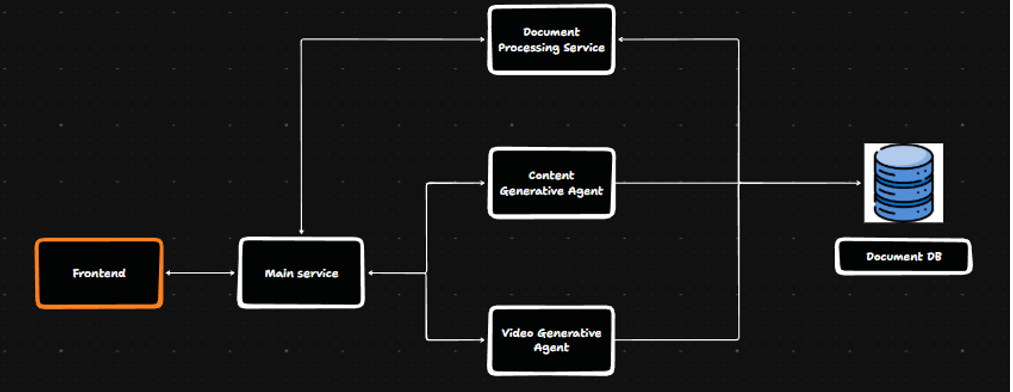
\includegraphics[width=0.7\textwidth]{images/kien-truc-tong-the.png}
    \caption{Kiến trúc tổng thể.}
    \label{fig:system-architecture}
\end{figure}

\subsection{Các thành phần chính của hệ
thống}\label{cuxe1c-thuxe0nh-phux1ea7n-chuxednh-cux1ee7a-hux1ec7-thux1ed1ng}

Hệ thống bao gồm các dịch vụ chuyên biệt được thiết kế để xử lý các chức
năng chính: quản lý tài liệu, truy xuất thông tin và tạo nội dung
marketing.

\begin{itemize}
\item
  Main Service (Dịch vụ chính)

  \begin{itemize}
  \item
    Đây là dịch vụ trung tâm chịu trách nhiệm xử lý tất cả các tương tác
    từ phía người dùng và điều phối các yêu cầu đến các dịch vụ khác.
  \item
    Chức năng:

    \begin{itemize}
    \item
      Xử lý các yêu cầu từ giao diện người dùng bao gồm xác thực, quản
      lý phiên người dùng và các thao tác cơ bản.
    \item
      Quản lý các tác vụ bất đồng bộ, bao gồm tạo, theo dõi và cung cấp
      trạng thái của các tác vụ đang thực hiện.
    \item
      Điều phối các yêu cầu đến các dịch vụ chuyên biệt và tổng hợp kết
      quả trả về cho người dùng.
    \item
      Cung cấp các API để quản lý tài liệu bao gồm upload, liệt kê và
      xóa tài liệu.
    \end{itemize}
  \end{itemize}
\item
  Document Processing Service (Dịch vụ xử lý tài liệu)

  \begin{itemize}
  \item
    Dịch vụ chuyên trách xử lý toàn bộ quy trình tiếp nhận, phân tích và
    lưu trữ tài liệu.
  \item
    Chức năng:

    \begin{itemize}
    \item
      Tiếp nhận tài liệu từ Main Service và thực hiện quá trình trích
      xuất văn bản từ các định dạng khác nhau (PDF, Word, Text, URL).
    \item
      Thực hiện phân đoạn văn bản (chunking) và tạo các vector embedding
      từ các đoạn văn bản.
    \item
      Lưu trữ các vector embedding vào Vector Database và lưu trữ
      metadata tài liệu vào Relational Database.
    \item
      Cung cấp thông tin trạng thái xử lý tài liệu để Main Service có
      thể theo dõi và thông báo cho người dùng.
    \end{itemize}
  \end{itemize}
\item
  Content Generative Agent (Tác nhân tạo nội dung)

  \begin{itemize}
  \item
    Dịch vụ chịu trách nhiệm thực hiện các tác vụ truy xuất thông tin và
    tạo nội dung marketing.
  \item
    Chức năng:

    \begin{itemize}
    \item
      Thực hiện truy xuất thông tin bằng cách chuyển đổi các truy vấn
      của người dùng thành vector, tìm kiếm các đoạn văn bản liên quan
      từ Vector Database và tạo câu trả lời dựa trên các đoạn văn bản
      được truy xuất.
    \item
      Tạo các nội dung marketing bao gồm caption, kịch bản video, chiến
      lược nội dung và các loại nội dung văn bản khác dựa trên các tài
      liệu đã được lưu trữ.
    \item
      Quản lý ngữ cảnh hội thoại để đảm bảo tính liên tục và nhất quán
      trong các tương tác liên tiếp.
    \end{itemize}
  \end{itemize}
\item
  Video Generative Agent (Tác nhân tạo video)

  \begin{itemize}
  \item
    Dịch vụ chuyên trách chuyển đổi kịch bản văn bản thành video hoàn
    chỉnh.
  \item
    Chức năng:

    \begin{itemize}
    \item
      Tiếp nhận kịch bản văn bản và các tham số tạo video từ Main
      Service.
    \item
      Thực hiện quá trình tạo video từ kịch bản bao gồm phân tích cấu
      trúc kịch bản, lựa chọn và ghép các thành phần hình ảnh, âm thanh
      và văn bản.
    \item
      Quản lý các tác vụ tạo video bất đồng bộ và cung cấp trạng thái xử
      lý cũng như kết quả video đã tạo.
    \item
      Xử lý các yêu cầu tùy chỉnh về phong cách, độ dài và các thành
      phần cụ thể của video.
    \end{itemize}
  \end{itemize}
\end{itemize}

Các dịch vụ này phối hợp với nhau thông qua Main Service, trong đó
Document Processing Service xử lý việc tiếp nhận và chuẩn bị dữ liệu,
Content Generative Agent thực hiện việc truy xuất thông tin và tạo nội
dung văn bản, Video Generative Agent tạo video từ các kịch bản văn bản,
và Main Service đảm bảo sự điều phối và quản lý toàn bộ quy trình tương
tác với người dùng.

Hệ thống sử dụng Vector Database để lưu trữ các embedding của tài liệu
và Relational Database để lưu trữ metadata tài liệu, thông tin người
dùng, trạng thái tác vụ và nội dung đã được tạo. Các tác vụ tạo nội dung
và video được xử lý bất đồng bộ với cơ chế theo dõi trạng thái để đảm
bảo người dùng có thể theo dõi tiến trình của các tác vụ mất nhiều thời
gian.

\subsection{Sơ đồ luồng dữ liệu tổng
quan}\label{sux1a1-ux111ux1ed3-luux1ed3ng-dux1eef-liux1ec7u-tux1ed5ng-quan}

\subsubsection{Nạp tri thức (Knowledge Ingestion Pipeline)}\label{so-do-nap-tri-thuc}

\begin{figure}[H]
    \centering
    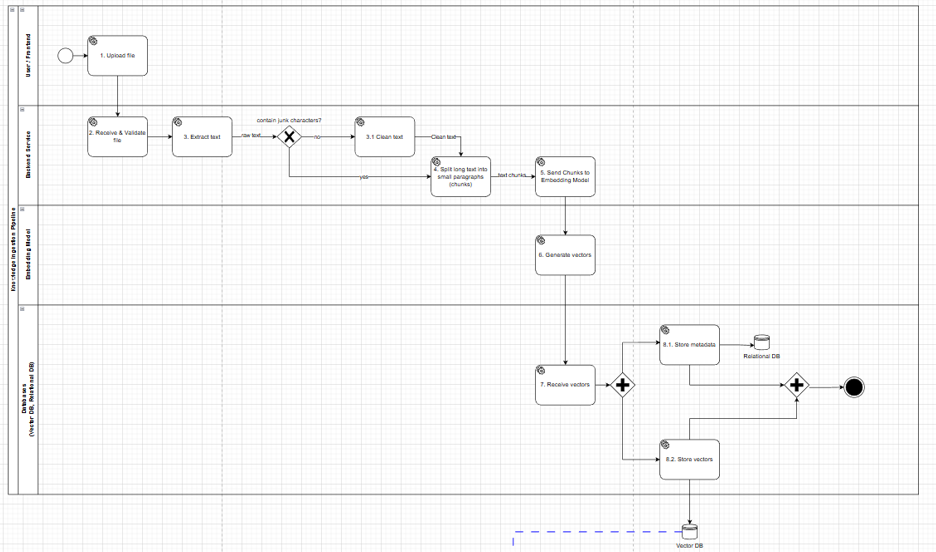
\includegraphics[width=0.7\textwidth]{images/so-do-du-lieu-nap-tri-thuc.png}
    \caption{Sơ đồ dữ liệu nạp tri thức.}
    \label{fig:knowledge-ingestion-flow}
\end{figure}

\begin{itemize}
\item
  Upload: Người dùng tải file lên từ Frontend -\textgreater{} Backend
  nhận file.
\item
  Extract \& Clean: Backend đọc nội dung file (Text extraction), loại bỏ
  ký tự rác.
\item
  Chunking: Chia văn bản dài thành các đoạn nhỏ (Chunks), ví dụ: 500
  từ/đoạn.
\item
  Embedding: Gửi các đoạn text này qua Embedding Model -\textgreater{}
  Nhận về các Vector.
\item
  Store: Lưu Vector vào Vector DB và lưu thông tin file (tên, ngày tạo)
  vào Relational DB.
\end{itemize}

\subsubsection{Truy xuất và Trả lời (Retrieval \& Generation Pipeline)}\label{try-xuat-va-tra-loi-cau-hoi}

\begin{figure}[H]
    \centering
    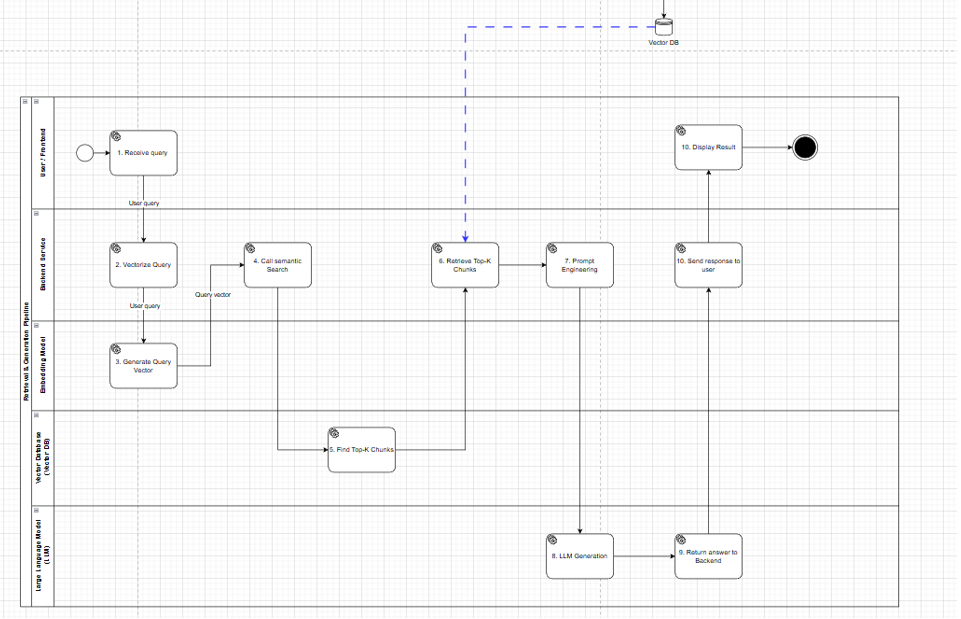
\includegraphics[width=0.7\textwidth]{images/so-do-du-lieu-tra-loi.png}
    \caption{Sơ đồ trả lời câu hỏi.}
    \label{fig:knowledge-ingestion-flow-detailed}
\end{figure}

\begin{itemize}
\item
  Receive Query: Người dùng đặt câu hỏi -\textgreater{} Backend nhận câu
  hỏi.
\item
  Vectorize Query: Chuyển câu hỏi thành Vector truy vấn.
\item
  Semantic Search: So sánh Vector truy vấn với hàng nghìn Vector trong
  Vector DB -\textgreater{} Tìm ra Top-K đoạn văn bản giống nhất
  (Relevant Chunks).
\item
  Prompt Engineering: Ghép "Câu hỏi" + "Top-K đoạn văn bản tìm được" vào
  một Prompt mẫu (System Prompt).
\item
  LLM Generation: Gửi Prompt trọn gói này tới LLM (OpenAI).
\item
  Response: LLM trả về câu trả lời tự nhiên -\textgreater{} Backend gửi
  về Frontend hiển thị cho người dùng.
\end{itemize}

\section{Thiết kế cơ sở dữ liệu sơ
bộ}\label{thiux1ebft-kux1ebf-cux1a1-sux1edf-dux1eef-liux1ec7u-sux1a1-bux1ed9}

\begin{figure}[H]
    \centering
    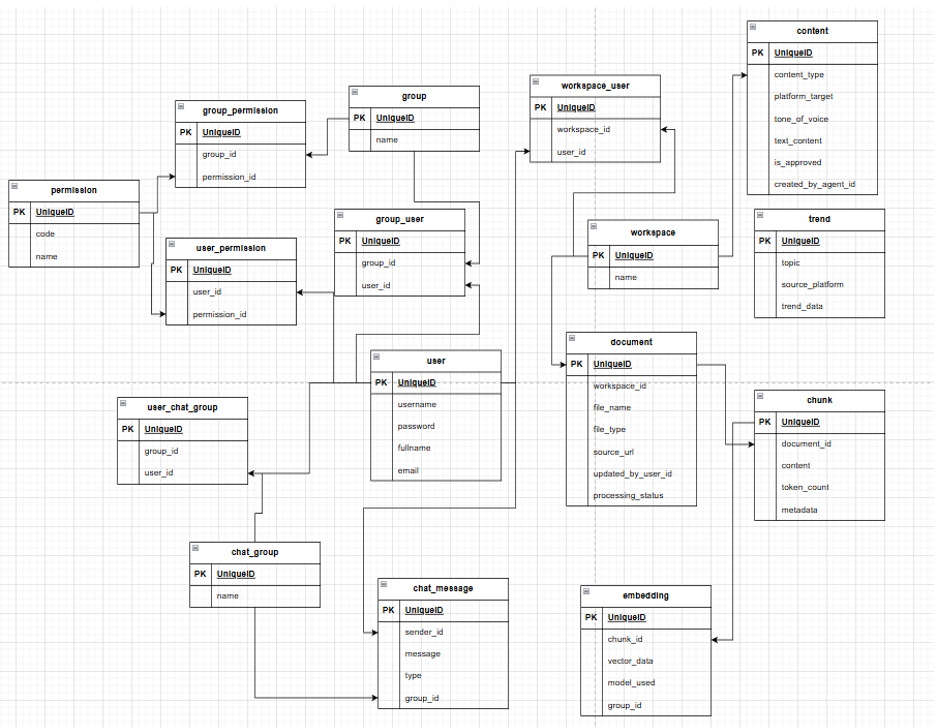
\includegraphics[width=0.7\textwidth]{images/co-so-du-lieu.png}
    \caption{Cơ sở dữ liệu.}
    \label{fig:database-schema}
\end{figure}

Cơ sở dữ liệu của hệ thống được thiết kế để quản lý toàn diện các thành
phần cần thiết cho việc vận hành AI Agent, bao gồm người dùng, phân
quyền, không gian làm việc, tài liệu và nội dung được tạo ra. Các bảng
chính trong cơ sở dữ liệu bao gồm:

\begin{enumerate}
\def\labelenumi{\arabic{enumi}.}
\item
  \textbf{Bảng User}: Lưu trữ thông tin về người dùng của hệ thống, bao
  gồm các thông tin cơ bản như tên đăng nhập, mật khẩu và thông tin cá
  nhân.
\item
  \textbf{Bảng Group}: Quản lý các nhóm người dùng, cho phép phân loại
  và quản lý người dùng theo các vai trò hoặc bộ phận khác nhau.
\item
  \textbf{Bảng Permission}: Định nghĩa các quyền hạn và các chức năng mà
  người dùng có thể thực hiện trong hệ thống.
\item
  \textbf{Bảng Group\_Permission}: Bảng trung gian liên kết giữa các
  nhóm người dùng và các quyền hạn, cho phép gán nhiều quyền hạn cho một
  nhóm và một quyền hạn có thể được gán cho nhiều nhóm.
\item
  \textbf{Bảng User\_Permission}: Bảng trung gian liên kết trực tiếp
  giữa người dùng và quyền hạn, cho phép phân quyền chi tiết cho từng
  người dùng cụ thể.
\item
  \textbf{Bảng Workspace}: Đại diện cho các không gian làm việc riêng
  biệt, mỗi không gian làm việc có thể chứa các tài liệu và nội dung
  riêng của một khách hàng hoặc một dự án cụ thể.
\item
  \textbf{Bảng Workspace\_User}: Bảng trung gian liên kết giữa người
  dùng và không gian làm việc, cho phép một người dùng tham gia vào
  nhiều không gian làm việc và một không gian làm việc có thể có nhiều
  người dùng.
\item
  \textbf{Bảng Group\_User}: Bảng trung gian liên kết giữa người dùng và
  các nhóm người dùng, cho phép một người dùng thuộc về nhiều nhóm và
  một nhóm có thể bao gồm nhiều người dùng.
\item
  \textbf{Bảng Document}: Lưu trữ thông tin về các tài liệu được người
  dùng tải lên hệ thống, phục vụ cho việc xây dựng cơ sở tri thức.
\item
  \textbf{Bảng Chunk}: Lưu trữ các đoạn văn bản được chia nhỏ từ các tài
  liệu. Mỗi tài liệu được phân chia thành các đoạn văn bản có kích thước
  phù hợp để xử lý và tạo embedding.
\item
  \textbf{Bảng Embedding}: Lưu trữ các vector biểu diễn số học của các
  đoạn văn bản (chunk), được sử dụng trong quá trình truy xuất thông tin
  dựa trên sự tương đồng ngữ nghĩa.
\item
  \textbf{Bảng Content}: Lưu trữ các nội dung được tạo ra bởi AI Agent,
  bao gồm các nội dung marketing, bài viết, kịch bản được sinh ra từ quá
  trình tương tác với hệ thống.
\item
  \textbf{Bảng Trend}: Lưu trữ thông tin về các xu hướng hoặc thông tin
  liên quan được sử dụng để định hướng việc tạo nội dung phù hợp với bối
  cảnh thị trường.
\item
  \textbf{Bảng Chat\_Group}: Quản lý các nhóm trò chuyện, cho phép tổ
  chức các phiên tương tác theo từng chủ đề hoặc dự án cụ thể.
\item
  \textbf{Bảng User\_Chat\_Group}: Bảng trung gian liên kết giữa người
  dùng và các nhóm trò chuyện, cho phép quản lý thành viên tham gia vào
  từng nhóm trò chuyện.
\item
  \textbf{Bảng Chat\_Message}: Lưu trữ lịch sử các cuộc trò chuyện giữa
  người dùng và AI Agent, bao gồm thông tin về người gửi, nội dung tin
  nhắn và nhóm trò chuyện tương ứng.
\end{enumerate}
